%
% 3-faltung.tex
%
% (c) 2022 Prof Dr Andreas Müller, OST Ostschweizer Fachhochschule
%
\section{Faltung
\label{buch:gruppen:section:faltung}}
\kopfrechts{Faltung}
Für einen Definitionsbereich $X$, der nur eine Menge ist, können
von Funktionen $f,g\in C(G)$ nur die Werte im gleichen Punkt
miteinander verglichen werden. 
Daher sind die einzigen algebraischen Operationen, die wir auf
$C(G)$ definieren können, die punktweise Addition $f+g$ und 
die punktweise Multiplikation $f\cdot g$ mit
\begin{align*}
(f+g)(x)      &= f(x)+g(x) \\
(f\cdot g)(x) &= f(x) g(x)
\end{align*}
Die Gruppenstruktur ermöglicht, verschiedene Punkte im Definitionsbereich
mit Hilfe einer Translation $T_x$ zur Deckung zu bringen und somit
Funktionswerte auf verschiedenen Gruppenelemente miteinander zu verrechnen.

%
% Hall
% 
\subsection{Hall und andere Phänomene, die auf die Faltung führen
\label{buch:gruppen:faltung:subsection:hall}}
\begin{figure}
\centering
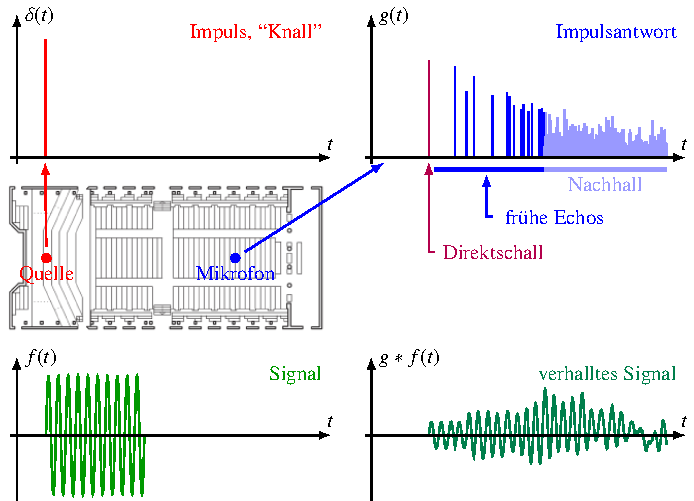
\includegraphics{chapters/030-gruppen/images/konzertsaal.pdf}
\caption{Echos und Nachhall in einem Konzertsaal.
Eine einzelner Impuls von einer Quelle (rot) führt beim Mikrofon
zu einer komplizierten Impulsantwort $g(t)$ bestehend aus
dem Direktschall, den frühen Echos und dem Nachhall.
Ein beliebiges Signal $f(t)$ (grün) wird beim Mikrofon als $g*f(t)$
aufgenommen.
\label{buch:gruppen:faltung:fig:konzertsaal}}
\end{figure}
Wie verändern die Reflexionen des Schalls in einem Konzertsaal
den Klang eines Musikinstruments
(Abbildung~\ref{buch:gruppen:faltung:fig:konzertsaal})?
Das Instrument produziert Schallwellen, die sich als Druckschwankungen
$f(t)$ ausbreiten.
Die Wände und Einrichtungsgegenstände reflektieren dies auftreffenden
Schallenwellen in unterschiedlichem Ausmass.
Die Reflexionen treffen beim Zuhörer mit verschiedenen Verzögerungen ein.
Das um $\tau$ verzögerte Signal ist $t\mapsto f(t-\tau)$.
Der Anteil $g(\tau)$ des Signals, des mit Verzögerung $\tau$ beim
Zuhörer eintrifft, heisst die {\em Impulsantwort}.
Das gesamte vom Zuhörer wahrgenommene Signal ist daher die Überlagerung
\begin{equation}
\int_{-\infty}^\infty
g(\tau) 
\,
f(t-\tau)
\,d\tau
\label{buch:gruppen:faltung:eqn:hall}
\end{equation}
all dieser Signale.
Das Integral wird auch als die Faltung $g*f$ bezeichnet.

Die Abbildung photographische mit einem realen Objektiv ist nicht
in der Lage, Punkte beliebig scharf abzubilden.
Stattdessen wird jeder Punkt auf ein Fleck abgebildet, dessen Intensität
mit zunehmender Entfernung vom idealen Bildpunkt abnimmt.
Dafür ist die Wellennatur des Lichts über das Phänomen der Beugung
verantwortlich.
Wir beschreiben das ideal abgebildete Bild als Funktion
$f\colon\mathbb{R}^2\to\mathbb{R}$.
Die Funktion $g(\xi)$ mit $\xi\in\mathbb{R}^2$ beschreibt die
Helligkeit des Flecks, der von einem Punkt erzeugt wird.
Die Helligkeit in einem Punkt $x$ des Bildes setzt sich zusammen
aus der Helligkeit $f(x-\xi)$ in Nachbarpunkten, gewichtet mit
$g(\xi)$, also
\begin{equation}
g*f(x)
=
\int_{\mathbb{R}^2} f(x-\xi)\,g(\xi)\,d\xi.
\label{buch:gruppen:faltung:eqn:pointspread}
\end{equation}
Im Kontext der Bildverarbeitung heisst
die Funktion $g(\xi)$ auch die {\em point spread function}.

%
% Faltung für Funktionen auf einer beliebigen Gruppe
%
\subsection{Faltung für Funktionen auf einer beliebigen Gruppe}
Die Integrale \eqref{buch:gruppen:faltung:eqn:hall} und
\eqref{buch:gruppen:faltung:eqn:pointspread} sind die Faltung
der Fuktionen $f$ und $g$.
Sie verwendet auf wesentliche Art die Gruppenstruktur des
Definitionsbereichs $\mathbb{R}$ der Funktionen.
Die Funktion $f(x-\xi)$ in \eqref{buch:gruppen:faltung:eqn:pointspread}
betrachtet als Funktion von $x$ ist die um $\xi$ verschobene
Funktion $T_\xi f(x)$.

Die obenstehenden Vorbereitungen können als
Ausgangspunkt für die Verallgemeinerung auf eine beliebige Gruppe
in der folgenden Definition verwendet werden.

\begin{definition}[Faltung]
Die Faltung zweier Funktion $f,g\in C(G)$ ist die Funktion
\begin{equation}
(f*g)(x)
=
\int_G f(y)g(y^{-1}x)\,dy.
\label{buch:gruppen:faltung:eqn:deffaltung}
\end{equation}
Im Fall einer additiv geschriebenen, abelschen Gruppe wird die Faltung zu
\begin{equation}
(f*g)(x)
=
\int_G f(y)g(x-y)\,dy.
\label{buch:gruppen:faltung:eqn:deffaltungadditiv}
\end{equation}
\end{definition}

In der Bestrebung, das Integral als Skalarprodukt von Funktionen
zu schreiben, dies muss der Faktor $g(x-y)$ als Funktion von $y$
ausgedrückt werden.

\begin{definition}
Zu einer Funktion $f\colon G\to X$ ist $\check{f}\colon G\to X$ die
Funktion mit den Werten $\check{f}(g) = f(g^{-1})$.
\end{definition}

Mit dieser Definition kann man
\[
T_s f(g)
=
f(s^{-1}g)
=
\check{f}(g^{-1}s)
=
T_g\check{f}(s)
\]
schreiben und damit das Faltungsintegral als
\[
\int_G g(\xi) T_\xi f(x)\,d\xi
=
\int_G g(\xi) T_x \check{f}(\xi)\,d\xi
=
\langle g, T_x\check{f}\rangle
\]
In dieser Form verschwindet das Integral im Skalarprodukt.


%
% Faltung als Produkt
%
\subsection{Faltung als Produkt
\label{buch:gruppen:faltung:subsection:produkt}}
Die Faltung ist ein Produkt, d.~h.~man kann mit Faltungsprodukten 
genau so rechnen, wie man es sich von anderen (nicht kommutativen)
Produkten wie zum Beispiel dem Matrizenprodukt gewöhnt ist.
Dazu müssen zwei Bedingungen erfüllt sein: es müssen das
Assoziativ- und das Distributivgesetz gelten.

%
% Assoziativität
%
\subsubsection{Assoziativität}
Das Assoziativgesetz besagt, dass es in einem Produkt mit mehr als
zwei Faktoren nicht auf die Reihenfolge ankommt, in der man die
Produkte ausführt.
Dies ermöglicht, Faltungsprodukte von drei Funktionen $f$, $g$ und $h$
auch einfach als $f*g*h$ zu schreiben.

\begin{satz}
Die Faltung ist assoziativ, also $(f*g)*h=f*(g*h)$ für Funktionen
$f,g,h\in C(G)$, für die alle Faltungen definiert sind.
\end{satz}

\begin{proof}[Beweis]
Ausgehend von der Definition der Faltung in
\eqref{buch:gruppen:faltung:eqn:deffaltung}
kann man den Wert der zweifachen Faltung als
\begin{align*}
((f*g)*h)(x)
&=
\int_G (f*g)(y) h(y^{-1}x)\,dy
=
\int_G \int_G f(z)g(z^{-1}y) \,dz\, h(y^{-1}x)\,dy
\intertext{berechnen.
Unter der postulierten Voraussetzung, dass alle Integrale existieren,
gilt der Satz von Fubini, der die Reihenfolge der Integrationen zu
vertauschen gestattet.
So wird die Faltung zu
}
&=
\int_G \int_G f(z)g(z^{-1}y) h(y^{-1}x) \,dy \,dz
\\
&=
\int_G f(z) \int_G g(z^{-1}y) h(y^{-1}x) \,dy \,dz
\intertext{Das Integral über $y$ ist invariant unter der Translation
mit $z$, wir schreiben daher $s=z^{-1}y$ und integrieren über $s$
statt $y=zs$:}
&=
\int_G f(z) \int_G g(s) h(s^{-1}z^{-1}x) \,ds \,dz
=
\int_G f(z) (g*h)(z^{-1}x) \,dz
=
(f*(g*h))(x)
\end{align*}
Damit ist die Assoziativität gezeigt.
\end{proof}

%
% Distributivität
%
\subsubsection{Distributivität}
Für ein Produkt wird zusätzlich erwartet, dass man damit rechnen kann
wie mit jedem anderen Produkt.
Dies bedeutet, dass für die Faltung und die Addition von Funktionen
das Distributivgesetz gilt, dass man also Faltungsprodukte
wie gewöhnliche punktweise Produkte von Funktionen
ausmultiplizieren und faktorisieren kann.

\begin{satz}
Für die Faltung und die Addition von Funktionen gilt das Distributivgesetz
\begin{equation}
\begin{aligned}
f*(g+h) &= f*g + f*h
&&\text{und}&
(f+g)*h &= f*h + g*h
\\
(\lambda f) * g &= \lambda (f*g) 
&&&
f*(\lambda f) &= \lambda (f*g).
\end{aligned}
\label{buch:gruppen:faltung:eqn:distributiv}
\end{equation}
\end{satz}

\begin{proof}[Beweis]
Das Distributivgesetz folgt sofort aus der Distributivität der Multiplikation
und der Linearität des Integrals:
\begin{align*}
(f*(g+h))(x)
&=
\int_G f(y) (g+h)(y^{-1}x)\,dy
\\
&=
\int_G f(y) g(y^{-1}x)\,dy
+
\int_G f(y) h(y^{-1}x)\,dy
=
(f*g)(x)
+
(f*h)(x)
\end{align*}
Die anderen Gleichungen \eqref{buch:gruppen:faltung:eqn:distributiv}
folgen auf die gleiche Art.
\end{proof}

%
% Kommutivität
%
\subsubsection{Kommutativität}
Die Faltung von Funktionen auf $\mathbb{R}$ mit der Addition ist
\begin{align*}
(f*g)(x)
&=
\int_{\mathbb{R}} f(y)g(x-y)\,dy
\intertext{mit der Substitution $s=x-y$ wird daraus}
&=
\int_{-\infty}^\infty f(x-s) g(s)\,ds
=
(g*f)(x).
\end{align*}
Das Faltungsprodukt von Funktionen auf $\mathbb{R}$ ist also kommutativ.
Dies gilt jedoch im allgemeinen nicht.

\begin{beispiel}
Die symmetrische Gruppe ist die kleinste nichtabelsche Gruppe.
Es gibt zwei Permutationen $\sigma$ und $\tau$, für die
$\sigma\tau\ne \tau\sigma$ gilt.
Wir berechnen die Faltung der beiden Funktionen 
\[
\raisebox{0.3cm}{$\displaystyle
\delta_\sigma(x) 
=
\begin{cases}
1&\qquad \text{falls $x=\sigma$}\\
0&\qquad \text{sonst}
\end{cases}
\qquad\text{und}\qquad
\delta_\tau(x) 
=
\begin{cases}
1&\qquad \text{falls $x=\tau$}\\
0&\qquad \text{sonst.}
\end{cases}$}
\qedhere
\]
\end{beispiel}

Man kann das auch noch etwas allgemeiner als in diesem Beispiel einer
endlichen Gruppe zeigen.
Dazu sei $G$ eine nichtabelsche Gruppe und $s,t\in G$ seien
zwei verschiedene Elemente, die nicht vertauschen, für die
also $st\ne ts$ ist.
Da die Verknüpfung in der Gruppe stetig ist, gibt es eine kleine
Umgebung $U$ des neutralen Elements derart, dass sich $sU$ und $tU$
nicht schneiden und auch keine gemeinsamen Punkte mit $stU$ und $tsU$, die
sich ebenfalls nicht schneiden.
Falls nicht, kann man die Umgebung $U$ immer noch kleiner machen, um
dies zu erreichen.
Sei ausserdem $f$ eine nichtnegative Funktion, deren Träger in $U$ enthalten
ist.
Wir rechnen jetzt nach, dass die Faltungen $T_sf*T_tf$ und $T_tf*T_sf$ 
nicht gleich sein können, was beweist, dass das Faltungsprodukt
nicht kommutativ sein kann.

Zu diesem Zweck untersuchen wir, wo die Faltung
\begin{equation}
(T_sf * T_tf)(x)
=
\int_G
T_sf(g) 
T_tf(g^{-1}x)
\,dg
=
\int_G
f(s^{-1}g)
f(t^{-1}g^{-1}x)
\,dg
\label{buch:gruppen:faltung:eqn:kommst}
\end{equation}
von $0$ verschieden sein kann.
Der erste Faktor ist höchstens in der Umgebung $sU$ von $0$ verschieden,
der zweite Faktor ist höchstens dann von $0$ verschieden, wenn
$t^{-1}g^{-1}x$ in der Nähe des neutralen Elementes ist.
Da $g$ in der Nähe von $s$ sein muss, ist $t^{-1}g^{-1}$ in der Nähe
von $t^{-1}s^{-1}=(st)^{-1}$.
Der zweite Faktor ist also höchstens dann von $0$ verschieden, wenn
$x$ in der Nähe von $st$ ist.
Der Träger der Faltung ist in einer Umgebung von $st$ enthalten.

Die Gruppenelemente $s$ und $t$ kommen in der Faltung
\eqref{buch:gruppen:faltung:eqn:kommst}
und in der nachfolgenden Diskussion symmetrisch vor.
Daraus folgt, dass die Faltung $T_sf*T_tf$ nur in einer Umgebung von $st$
von $0$ verschieden ist, während $T_tf*T_sf$ nur einer davon disjunkten
Umgebung von $ts\ne st$ von $0$ verschieden ist.
Die beiden Funktionen $T_sf*T_tf$ und $T_tf*T_sf$ können daher
nicht gleich sein, die Faltung ist nicht kommutativ.

%
% Rekonstruktion der Gruppenoperation aus der Faltung
%
\subsubsection{Rekonstruktion der Gruppenoperation aus der Faltung}
Die Diskussion zeigt auch, dass man die Verknüpfung in der Gruppe aus
der Faltung rekonstruieren kann.
Gegeben zwei Elemente $s,t\in G$ und Funktionen $f_n$,
deren Träger in einer Umgebung des neutralen Elementes
enthalten sind, und die für grösser werdendes $n$ schnell kleiner werden..
Dann zeigt die Diskussion oben, dass der Träger der Faltung 
$T_sf_{\varepsilon}*T_tf_{\varepsilon}$ in einer Umgebung von $st$
enthalten sein muss.
Der Träger von $T_sf_n*T_tf_n$ wird kleiner, je grösser man $n$ macht.
Wählt man für jedes $n$ ein Element $g_n$ im Träger der Faltung,
entsteht eine Folge in $G$, die gegen $st$ konvergiert.

Statt die Gruppe und ihre Elemente zu studieren, kann man also die
gleichen Informationen auch aus dem Studium der Faltung von Funktionen
auf der Gruppe gewinnen.
Der Vorteil des Zugangs über Funktionen auf der Gruppe besteht
darin, dass Funktionen einen Vektorraum bilden, auf dem zwei
verschiedene Multiplikationen definiert sind.
Das Skalarprodukt sorgt zusätzlich dafür, dass die quadratintegrierbaren
Funktionen einen Hilbert-Raum bilden.
Diese zusätzlichen algebraischen Strukturelemente geben uns weitere
Werkzeuge in die Hand, die Gruppe zu studieren.







